\begin{figure}
	\centering
	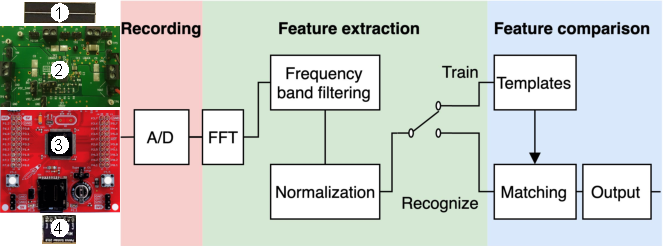
\includegraphics[width=\columnwidth]{figures/cis}
	\caption{Coalesced Intermittent Command Recognizer: an instant of a \fullsys. On the left is the hardware of an individual intermittent sensory node. Our prototype consists of 8 coalesced intermittent nodes. \circled{1} is an SLMD121H04L solar panel. \circled{2} is a BQ25570EVM-206 solar power harvester, \circled{3} is an MSP430FR5994 ultra low power microcontroller, and \circled{4} is a home soldered PCB with KPMM-3738-VM1010-R microphone. The block diagram on the right shows the data acquisition and processing stages.}
	\label{fig:powerCycle}
\end{figure}

We have developed a prototype of a \fullcim (\cim): an instant of a \fullsys. The reason behind developing a \cim is threefold: (i) voice is a natural and convenient way for human to interact with miniaturized devices; (ii) By demonstrating \textit{the world's first} \fullcim, we are shading light on the potential of intermittent systems; and (iii) it facilitates testing with different sensing strategies and with different type of external events arrival (i.e. regular  or burst). 

We envision that a \cim can be embedded in clothes, walls, wallpapers, and furniture coverage. \cim can enable local communication by taking advantage of the recent advancements in passive communication (\cite{marco} shows 60\,m distance of direct passive light communication). 

\subsection{Hardware}
A \cim node consists of thee main parts: a microphone, a microcontroller, and a harvester. we used MSP430RF5994~\cite{ti_msp430_website} an ultra-low-power microcontroller for data acquisition and processing. This microcontroller has a 16-bit RISC processor running on 1 MHz, 8KB of SRAM (volatile), 256KB of FRAM (non-volatile), and a 12-bit analog to digital converter (ADC). It also features a Low Energy Accelerator (LEA), which offloads the main CPU for specific operations, such as FFT. For recording we used the PMM-3738-VM1010-R piezoelectric MEMS microphone, which features Wake on Sound and ZeroPower listening technologies \cite{microphone}, allowing both the microcontroller and the microphone to sleep in a low-power mode until a sound is detected.
The microcontroller and microphone are powered by a BQ25570 solar power harvester~\cite{BQ25570EVM-206_website} connected to an IXYS SLMD121H04L solar cell~\cite{SLMD121H04L_website} and a super-capacitor of 220 \si{\micro F}. For debugging we used the Saleae logic analyzer~\cite{saleae}.

\subsection{Data acquisition}
To cover the frequency range of the human voice, we used a sample rate of 7,812 Hz. To determine the location of the word within the recorded signal, we relied on the microphone feature  \textit{Wake-on-sound} and on the characteristics of the targeted vocabulary. The wake-on-sound triggers the data recording on the beginning of a word---once the energy in the sound wave crosses a certain level the recording begins. Experimentally, we defined the effective recoding length to be 259\,ms. Thus, endpoint detection algorithm is not needed, greatly improving the processing time and system efficiency from the energy perspective.

only trigger the recording process after the energy in the sound wave crosses a certain threshold

By studying the characteristics of the targeted vocabulary -- in particular the minimum effective recording length (\cref{sec:rec_length}) -- we selected a fixed recording length of 295 ms. Because we used a fixed recording length and exploited the \textit{wake-on-sound} microphone feature, the position of the word in the recording is always the same and endpoint detection is not needed, greatly improving the processing time and system efficiency from the energy perspective.

Once a recording has finished, framing and data processing begin. We used non-overlapping frames of 256 samples ($\approx$ 33 milliseconds). This size is beneficial for doing a Fast Fourier Transform and short enough for the voice-features to be considered constant inside one frame (see \cref{sec:speech_recognition}).

% \begin{figure}
% 	\centering
% 	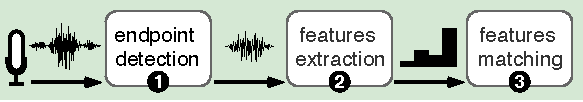
\includegraphics[width=\columnwidth]{figures/distributedMicrophone}
% 	\caption{ (1) endpoint detection algorithms extract the part of the signal corresponds to the input word, (2) feature extraction calculates the energy spectrum of the trimmed signal, and (3) feature matching searches the local database for the closest word}
% 	\label{fig:mic}
% \end{figure}

\subsection{Software}

%\textit{Endpoint detection} determines if there is a word in the recorded audio sample and, if there indeed is, the location of the word inside the recording is determined. There are several methods for doing endpoint detection. Two of them have been implemented and tested: power based and zero crossing rate (ZCR) based. The power based method estimates the energy of the audio signal by calculating the sum of amplitudes squared ($E = \sum A^2$) for each frame. The ZCR method counts how often the zero line is crossed per frame. The zero line in this case is equal to the microphone offset.

During \textit{feature extraction} on frames containing the word Fast Fourier Transform is applied to obtain the energy spectrum. 
The energy spectrum is then sorted into a feature vector, where each vector value holds the total energy of a specific frequency range. Finally each vector value is normalized over the total vector energy.

After that, \textit{feature matching} is performed, where the features of the recorded word are compared against a local database to find the most similar word in the database.
There exist many feature matching methods, yet only few are able to run under the constraints of an intermittent system.
Two methods have been implemented and tested. The first is Dynamic Time Warping (DTW), which is able to compare two sequences of data, even when they vary in speed. This way if a word is spoken slower or faster, the algorithm can compensate for that.
The second is a method that linearly compares two feature vectors. This requires less computations than DTW.


\subsection{Implementation}
During recording a sample rate was used of 7812 Hz, which covers the human voice frequency range. The used frame size was 256 samples. This size was beneficial for doing a Fast Fourier Transform and corresponds to approximately 33 milliseconds of speech.

For normalization an integer log function was applied on every value, divided by the average log.
The whole algorithm is implemented using only integer / fixed point arithmetic.

%DTW is a well known method in speech recognition.
In the linear comparing method the feature vectors of two words are compared successively, not accounting for differences in the speed of pronunciation. If two words vary in length, the last frames cannot always be compared and instead a penalty is applied linear to the length difference.

In between the different steps (see figure \ref{fig:mic}) checkpoints in non-volatile memory are used to assure progress while running on intermittent power. In some cases additional checkpoint were used inside the steps.

